\documentclass[twocolumn]{article}
\usepackage[left=48pt,right=46pt]{geometry}
\date{}
\usepackage{polyglossia}
\setmainfont{Cambria}
\setmonofont{Liberation Mono}
\setmainlanguage{english} % can be changed to desired language
\bibliographystyle{vancouver}
\usepackage{microtype}
\usepackage{rotating}
\usepackage{caption}
\usepackage{authblk}
\usepackage{indentfirst}
\usepackage{threeparttable}
\usepackage{tablefootnote}
\usepackage{graphicx}
\usepackage{multirow}
\usepackage{longtable}
\usepackage{wrapfig}
\usepackage{array}
\usepackage{booktabs,siunitx}
\usepackage{mathtext}
\usepackage[hyphens]{url}
\urlstyle{same}
\usepackage{lineno,hyperref}
\usepackage{tabulary}
\modulolinenumbers[5]
\usepackage{fancyhdr}
\pagestyle{fancy}
\fancyhead{}
\fancyfoot[C]{\thepage}
\fancyhead[C]{Psychosomatic Medicine and General Practice $\bullet$ March 2017 $\bullet$  V. 2, I. 1 $\bullet$ e020126}
\fancyfoot[RO,LE]{}
\setlength\parindent{20pt}
\setlength{\parskip}{2pt}
\begin{document}
\title{
\smash{\includegraphics[scale=0.15]{logo}}\\[-1.5cm]
\bfseries \qquad Psychosomatic Medicine and General Practice\\[0.5cm]{
\flushleft\small{DOI: someDoiIndex\hfill }\\[0.4cm]
\flushleft\small{UDC: 612.821.1\hfill }\\[0.4cm]}{
\LARGE \bfseries Evaluation of the evoked brain potentials of patients with asthenia and anxiety symptoms and the partial lost of sight
}}
\author[1,2,3]{Tsira A.}
\author[2,3]{Ruslan A.}
\author[3]{Andriy S.}
\author[4]{Katherine K.}
\author[4]{Inna M.}
\affil[1]{Ukrainian Research Institute of Social and Forensic Psychiatry and Drug Abuse}
\affil[2]{Eye Microsurgery Center}
\affil[3]{Donetsk National Medical University}
\affil[4]{Bogomolets National Medical University}
\twocolumn[
\begin{@twocolumnfalse}
\maketitle
\begin{center}
{\Large \textbf{Abstract}} \vspace{1ex}\\
\end{center}
\textbf{Background. }Loss of sight, even partial, especially in adulthood, is accompanied by emotional, motivational and social consequences that directly affect the psychophysiological state of the individual himself, his communication in society and, often, the social status of the subject. \vspace{1ex}\\
\textbf{Methods. }From the group of patients-volunteers (n=15) with a partial loss of sight of traumatic genesis two groups were formed for carrying out neurophysiological studies: with predominant asthenia and predominant anxiety. The controle group (CG) constisted from patients of the same age (n=20) without psychiatric comorbidity. A study of acoustic event-related potentials of the brain (ERP) was carried out in the oddball paradigm with the recording of the time and correctness of a simple sensorimotor reaction. \vspace{1ex}\\
\textbf{Results. }Comparative analysis of the asthenia group with the comparison group revealed a sufficient number of indicators of the ERP, which have significant statistical differences. The correctness of the sensorimotor reaction in this group was 98.3 $\pm$ 2.44\%, whereas in the CG - 92.5 $\pm$ 5.74\% (U = 62.5, p \textless{}0.01). The values of the amplitude of the early positivity of P1 in the asthenia group were 4.25 $\pm$ 3.312 $\mu$V, and in the CG -4.15 $\pm$ 7.933 $\mu$V (U = 50, p \textless{}0.001). The early negativity in that group was -2.78 $\pm$ 2.377 $\mu$V, and in the CG it was 10.55 $\pm$ 7.466 $\mu$V (U = 75; p \textless{}0.05). \vspace{1ex}\\
\textbf{Conclusion. }In the asthenia group this is the correctness of the sensorimotor reaction and the amplitude of the components: P1, N1, P2, N2. In the anxiety group, such indicators were: latency period P1, intervals P1N1 and N2P3, amplitude swing P1N1. A specific marker of the asthenia group, distinguishing it from the CG, was the more positive values of the amplitude of the components P1, N1, P2, N2. Taking into account the low-frequency nature of the modulation of the amplitudes of these components (circa 2 Hz), it can be assumed that nonspecific brainstem systems are involved in the process. \vspace{1ex}\\
{\textbf{Ключові слова:}} \texttt{loss of sight}, 
\texttt{trauma}, 
\texttt{nonpsychotic}, 
\texttt{mental disorders}, 
\texttt{asthenia}, 
\texttt{anxiety}, 
\texttt{neurophysiology}, 
\texttt{cognitive}, 
\texttt{evoked potentials}, 
\texttt{brain}, 
\texttt{sensorimotor reaction}\vspace{5ex}
\end{@twocolumnfalse}]
\section{Background}
\par The visual analyzer is the main sensory channel for humans that connects them with the environment. And therefore, loss of sight, especially in adulthood, is accompanied by emotional, motivational and social consequences that directly affect the psychophysiological state of the individual himself, his communication in society and, often, the social status of the subject\cite{bib1}. In 90\% of cases of vision loss, this condition is accompanied by depression due to disability\cite{bib2}, and in case of loss of sight of traumatic genesis, this process is further exacerbated by negative psychopathological manifestations, caused by the additional aggravating effect of posttraumatic stress on the state of mental health of a person\cite{bib3},\cite{bib4},\cite{bib5},\cite{bib6},\cite{bib7}. The obvious relevance of the problem implies the involvement of various approaches to its solution, and the neurophysiological approach, as we hope, will allow us to identify new neurophysiological predictors for effective diagnosis and treatment of these disorders, on the one hand, and on the other hand - to elucidate the physiological mechanisms of these conditions. Earlier our group carried out neurophysiological studies of patients with nonpsychotic mental disorders due to a partial loss of sight owed to trauma\cite{bib8}. However, later we assumed that the group of patients, that was studied by us is not homogeneous, which made us take a more differentiated approach. The results of these studies are presented in this paper.
\section{Methods}
\par Comprehensive studies were carried out on the basis of the department of eye trauma, as well as the office of urgent care for eye trauma during 2010-2013. Studies were conducted with the obligatory observance of the principles of bioethics and deontology. The volunteer patients were informed of the nature and purpose of the studies and consent for research was obtained from them. A randomized group of subjects was formed in the period after the ophthalmologic intervention and determination of the volume and prognosis of sight loss. A total of 600 people with partial loss of sight of traumatic genesis (PLVTG) underwent a screening examination. The manifestations of an acute stress reaction were recorded in all patients. Within one to three months after discharge from the hospital, when patients underwent MSE, we conducted an in-depth clinical-psychopathological examination of patients. As a result two groups of research were formed: the main group (MG) - 200 Patients who, after a traumatic event that caused a partial loss of sight, were diagnosed with nonpsychotic mental disorders (NPD), and a comparison group (CG) - 200 people whose mental state was consistent with the so-called "conditional norm". The criteria for exclusion from the study were lack of informed consent, history of mental and behavioral disorders, and the presence of severe somatic diseases, during which the patient's mental state may be affected.
\par Clinical-psychopathological research was conducted through an in-depth clinical standardized interview using ICD-10 diagnostic criteria. A subjective evaluation of the available clinical and psychopathological manifestations was carried out using the Beck depression inventory\cite{bib9}, diagnostic techniques for self-assessment of reactive (R) and personal (P) anxiety of Ch. D. Spielberger-Y. L. Khanin\cite{bib10}. The analysis of objective manifestations of psychopathological symptoms was carried out using Hamilton’s clinical rating scales of depression (D) and anxiety (A) HDRS and NARS\cite{bib11}. The nosological structure of diagnosed NPD was represented by mental and behavioral disorders of cluster F43 - "response to stress and adaptive disorders" (22\%), adaptation disorders with a predominance of disturbances of other emotions F43.23 (14.5\%); Post-traumatic stress disorder F43.1 (11.5\%), adaptation disorder with mixed emotions and behavior disorder F43.25 (3.5\%).
\par Two groups were formed to carry out electrophysiological studies to identify the characteristics of neurophysiological mechanisms of the development of NDP owed to PLVTG from the MG: asthenia and anxiety, which included 15 men aged 22 to 57 years, and a CG of 20 men of men of the same age. The asthenia group included patients with a clinical prevalence of asthenia, in whom asthenic-depressive and asthenic-hypochondriac syndromes were identified. The anxiety group included patients with a clinical prevalence of anxiety with anxiety-depressive, anxious-phobic and obsessive-phobic syndromes.
\par Electrophysiological studies were carried out using the diagnostic complex "Amplaid MK15" (Italy). To study brain electrical activity, the method of event-related evoked potentials (ERP) was used of auditory modality. Which was connected with the asthenia and anxiety features of the tested groups, that had a disruption of the function of the visual system. The subject was binaurally presented with a series of stimuli in the pseudo-random (with a predetermined probability of the appearance of significant stimuli) sequence – oddball paradigm. A significant stimulus - a tone with a frequency of 4000 Hz was presented with a probability of 20\%, a background stimulus - tone with a frequency of 1000 Hz was presented with a probability of 80\%. The intensity of the sounds was 100 dB above the threshold of audibility\cite{bib12}. The interval between stimuli was 2 seconds. The subject was instructed to react to the appearance of a significant signal by pressing the button, background stimuli were ignored. When the button was pressed, registration of the induced brain electrical activity occurred, as well as the time and correctness of a simple sensorimotor reaction. The registration of the ERP was carried out from the head surface with standard electroencephalographic electrodes located in the 10/20 (Jasper) system at the points: Cz - active electrode, A1 + A2 - common refractive electrode, Fpz – grounding electrode. The averaging of evoked potential was carried out based on 100 records\cite{bib13}. Elimination of artifacts, including eye movement artifacts, was hardware-based. The components of P1, N1, P2, N2, P3 and N4 were marked out on the ERP curve registered for a significant stimulus (Fig. \ref{fig1}). The positive component in the range of latent periods from 30 to 80 ms was regarded as P1, negativity from 80 to 140 ms - as N1, the positive component of P2 was differentiated in the time interval 120-200 ms, N2 - between 180 and 320 ms from the start of the scan, and the late positive component P3 was detected in the range of 270-550 ms, and the next maximum negative bias potential was considered as component N4. Statistical software package Statistica 5.5 (StatSoft, USA) was used for statistical processing of the obtained experimental results. When checking statistical hypotheses, the values of criteria with significance level p \textless{}0.05 were considered reliable. The comparative analysis was carried out by nonparametric methods: the Wilcoxon T-test and the Man-Whitney U test, and the Pearson-Spearman correlation analysis\cite{bib14}.
\begin{figure}
\caption{Acoustic ERP in the comparison group, in the main group and in asthenia group.}
\label{fig1}
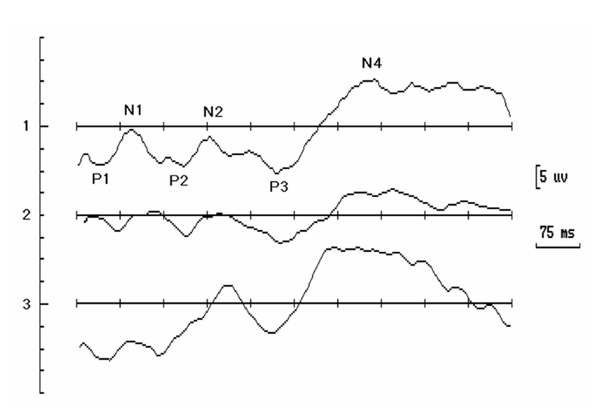
\includegraphics[width=\linewidth ]{fig1.png}
\caption*{*The main components of the curve (P1, N1, P2, N2, P3, N4), whose indices were analyzed, are indicated. Positive deviation of the potential goes down.}
\end{figure}
\section{Results}
\subsection{The results of psychological testing in asthenia and anxiety groups}
\par The results of psychological testing show the differences between the groups in all indicators: RA, PA, Ds, Do, Ao (Fig. \ref{fig2}). At the same time, the values of the three parameters - RA, PA and Do in the anxiety group were higher than in the asthenia group. Thus, the RA index in the anxiety group (59.3 $\pm$ 2.13) was higher (U\cite{bib15}= 0; p \textless{}0.001) than in the asthenia group (49.7 $\pm$ 2.12). PA in the anxiety group (46.7 $\pm$ 3.81) also exceeded (U = 25, p \textless{}0.001) the values of the asthenia group (35.0 $\pm$ 6.92), and the Ao values in the anxiety group (22,0 $\pm$ 0.85) were almost twice as large (U = 0, p \textless{}0.001) than in the asthenia group (13.3 $\pm$ 2.97). The two remaining indicators: Ds (16.0 $\pm$ 0.84) and Do (17.7 $\pm$ 1.76) in the anxiety group were lower than in the asthenia group - 20.3 $\pm$ 2.58 (U = 12.5, p \textless{}0.001) and 24.67 $\pm$ 1.76 (U = 0; p \textless{}0.001) respectively.
\begin{figure*}
\caption{The values of indicators of RA, PA, Ds, Do and Ao in the main asthenia and anxiety groups of subjects and in comparison group.}
\label{fig2}
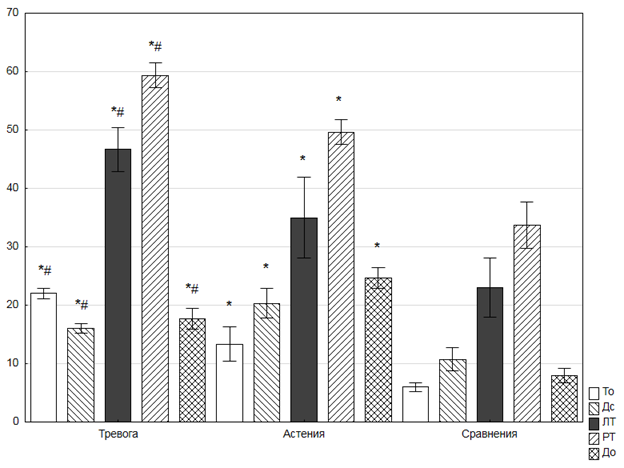
\includegraphics[width=\linewidth ]{fig2.png}
\caption*{* - differences with significance level of p\textless{}0,05. \# - significant differences (p \textless{}0.05) in comparison with the asthenia group and * - with the comparison group.}
\end{figure*}
\par The indices of psychological testing of asthenia and anxiety groups showed significant exceeding values (U values\cite{bib15},\cite{bib20}from 0 to 25, p \textless{}0.001) of RA, PA, Ds, Do and Ao of both groups relative towards the comparison group (Fig. \ref{fig2}).
\subsection{	ERP in the asthenia and anxiety groups}
\par Comparative analysis of cognitive evoked potentials in anxiety and asthenia groups revealed a number of statistically significant differences (Fig. \ref{fig3}). The time of the sensorimotor reaction in the anxiety group was 337.3 $\pm$ 9.31 ms, which was significantly higher (U\cite{bib15};\cite{bib15}= 50; p \textless{}0.05) than in the asthenia group (308.7 $\pm$ 31.28 ms ). The latent period of the P1 component of the ERP in the anxiety group (76.0 $\pm$ 23.42 ms) significantly exceeded (U\cite{bib15};\cite{bib15}= 50, p \textless{}0.05) the latent period of this component in the asthenia group (52.3 $\pm$ 31 , 28 ms).
\begin{figure}
\caption{Time parameters of the ERP.}
\label{fig3}
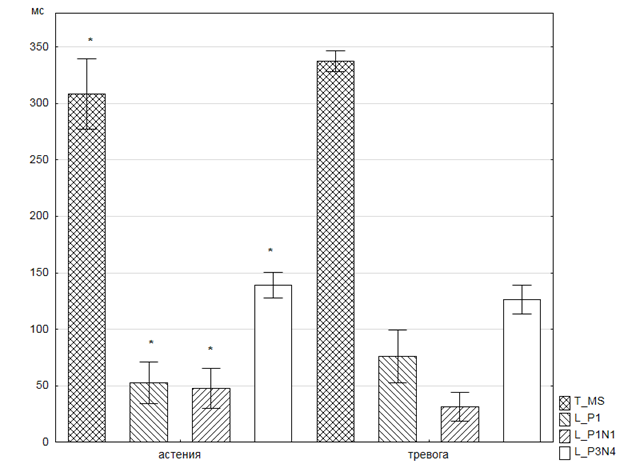
\includegraphics[width=\linewidth ]{fig3.png}
\caption*{*Time parameters of the ERP: time of sensorimotor reaction (T\textunderscore{}ms), latent period of component P1, inter-peak intervals P1N1 and P3N4 in asthenia and anxiety groups. Medium values and standard deviations are presented. * - significant differences (p \textless{}0,05) in the studied groups.}
\end{figure}
\par The amplitude of the negative N2 component in the anxiety group (-6.54 $\pm$ 2.261 $\mu$V) had more negative values than in the asthenia group (-1.23 $\pm$ 1.644 $\mu$V) (U\cite{bib15}= 0; p \textless{}0.001). The temporal indices of the ERP, such as the intervals P1N1 and P3N4, were smaler than in the asthenia group. Thus, the values of the P1N1 interval in the anxiety group were 31.0 $\pm$ 12.76 ms, and in the asthenia group they were 47.7 $\pm$ 17.94 ms (U\cite{bib15},\cite{bib15}= 50, p \textless{}0.05). And the interval of the later P3N4 complex  in the anxiety group was longer than in the early complexes and equaled 126.0 $\pm$ 12.68 ms, which was less than in the asthenia group 139.0 $\pm$ 11.43 ms (U\cite{bib15},\cite{bib15}] = 62.5, p \textless{}0.05).
\subsection{ERP in asthenia and anxiety groups compared to the control group }
\par Comparative analysis of the asthenia group with the comparison group revealed a sufficient number of indicators of the ERP, which have significant statistical differences. The correctness of the sensorimotor reaction in this group was 98.3 $\pm$ 2.44\%, whereas in the CG - 92.5 $\pm$ 5.74\% (U\cite{bib15},\cite{bib20}= 62.5, p \textless{}0.01). Also in this group there were differences in the amplitudes of the components: P1, N1, P2, N2 (Fig. \ref{fig4},Fig. \ref{fig5}). So, the values of the amplitude of the early positivity of P1 in the asthenia group were 4.25 $\pm$ 3.312 $\mu$V, and in the CG -4.15 $\pm$ 7.933 $\mu$V (U\cite{bib15},\cite{bib20}= 50, p \textless{}0.001). The early negativity in that group was -2.78 $\pm$ 2.377 $\mu$V, and in the CG it was 10.55 $\pm$ 7.466 $\mu$V (U\cite{bib15},\cite{bib20}= 75; p \textless{}0.05). Differences between late P2 and N2 have the same trend of differences for the compared groups. The P2 values were 3.40 $\pm$ 2.029 $\mu$V in the asthenia group and -3.08 $\pm$ 8.287 $\mu$V in the CG (U\cite{bib15},\cite{bib20}= 75; p \textless{}0.05), the N2 value was -1.23 $\pm$ 1.644 $\mu$V , and in the CG it was 7.23 $\pm$ 5.754 $\mu$V (U\cite{bib15},\cite{bib20}= 75; p \textless{}0.05). In the anxiety group, there were other, different from the asthenia group, significant indicators of the ERP. Basically, these were time indicators, such as the latency period of the P1 component, which values in the anxiety group were 76.0 $\pm$ 23.42 ms, while in the CG they were 49.3 $\pm$ 4.38 ms (U\cite{bib15},\cite{bib20}= 0 ; P \textless{}0.001), as well as P1N1 intervals of 31.0 $\pm$ 12.76 ms in the anxiety group and 58.8 $\pm$ 7.447 ms in the CG (U\cite{bib15},\cite{bib20}= 0; p \textless{}0.001).
\begin{figure}
\caption{Amplitudes of positive components of ERP P1, P2, N1P2, P3N4 in the anxiety, asthenia and comparison groups.}
\label{fig4}
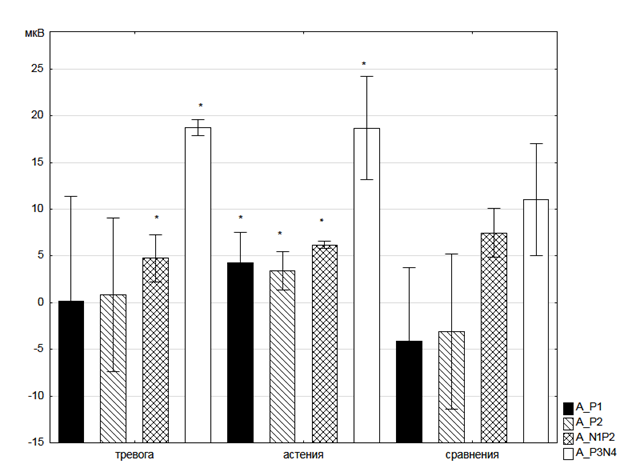
\includegraphics[width=\linewidth ]{fig4.png}
\caption*{*significant differences (p \textless{}0.05) of the indicators compared to the comparison group}
\end{figure}
\par The interval of late N2P3 components in the anxiety group was 103.0 $\pm$ 24.09 ms, and in the CG it was 150.0 $\pm$ 48.812 ms (U\cite{bib15};\cite{bib20}= 75; p \textless{}0.05). In addition to the P1N1 interval in the anxiety group, significant differences from the CG showed the  P1N1 amplitude swing, which was 31.0 $\pm$ 12.76 $\mu$V, whereas in the CG it was 6.39 $\pm$ 1.110 $\mu$V (U\cite{bib15};\cite{bib20}= 50; P \textless{}0.001). Among the indicators of the ERP were also those that had statistically significant differences from CG in both groups.
\begin{figure}
\caption{Amplitudes of negative components of ERP N1, N2, N4 in anxiety, asthenia and comparison groups.}
\label{fig5}
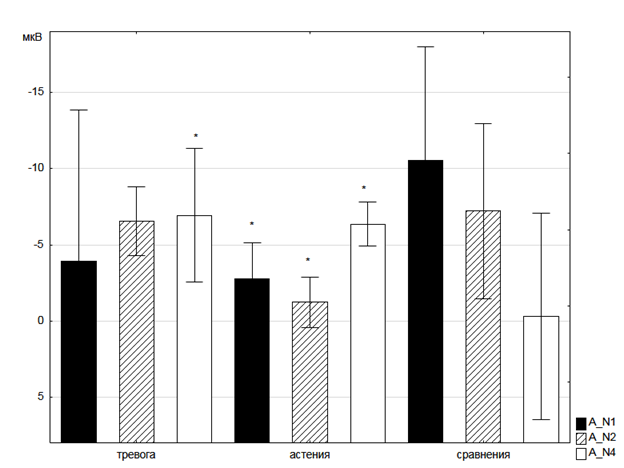
\includegraphics[width=\linewidth ]{fig5.png}
\caption*{*significant differences (p \textless{}0.05) of the indicators compared to the comparison group.}
\end{figure}
\par These include such ERP indicators as latent periods of P3 and N4 components, amplitude N4 and amplitude ranges of N1P2 and P3N4. The latent periods of the P3 component and in the asthenia group are 312.0 $\pm$ 33.16 ms (U = 50; p \textless{}0.001), and in the anxiety group 320.0 $\pm$ 34.61 ms (U\cite{bib15};\cite{bib20}= 87.5, p \textless{}0.05) were lower than in the CG (368.3 $\pm$ 37.15 ms) (Fig. \ref{fig6}). The latent periods of component N4 and in the asthenia group (451.0 $\pm$ 33.09 ms, (U = 25; p \textless{}0.001)), and in the anxiety group (446.0 $\pm$ 25.52 ms, (U = 50; p \textless{}0.001)) were lower than the values of this component in the CG (498.8 $\pm$ 32.67 ms). Amplitudes of this component had more negative values: -6.36 $\pm$ 1.44 $\mu$V (U = 75; p \textless{}0.05) - in the asthenia group, -6.93 $\pm$ 4.379 $\mu$V (U = 50, p \textless{}0.001) - in the anxiety group compared to the CG, where its values were -0.29 $\pm$ 6.789 $\mu$V. If the amplitude of the N1P2 amplitudes in the asthenia group (6.19 $\pm$ 0.416 $\mu$V (U = 75; p \textless{}0.05)) and anxiety group (4.75 $\pm$ 2.538 $\mu$V (U = 50; P \textless{}0.001)) were smaller than the CG (7.47 $\pm$ 2.599 $\mu$V), when the amplitude of the later P3N4 was 18.69 $\pm$ 5.525 $\mu$V (U = 25; p \textless{}0.001) and 18.75 $\pm$ 0.873 MV (U = 75; p \textless{}0.05), respectively, exceeded the values of CG (11.04 $\pm$ 5.965 $\mu$V).
\begin{figure}
\caption{\textbf{Figure 6}. Time parameters of ERP: latent periods of P1, P3, N4 components and P1N1, N2P3 intervals in anxiety, asthenia and comparison groups.}
\label{fig6}
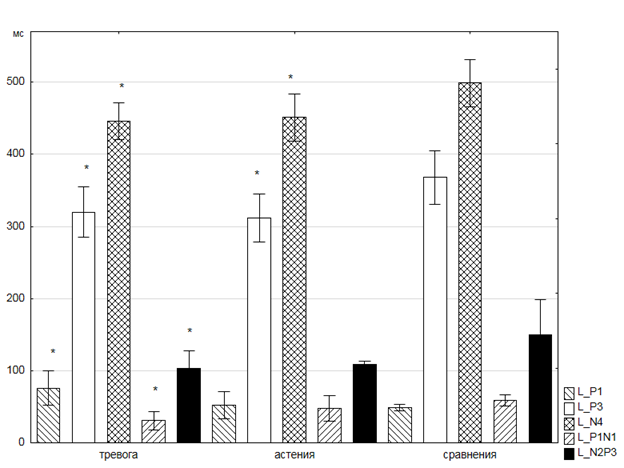
\includegraphics[width=\linewidth ]{fig6.png}
\caption*{*significant differences (p \textless{}0.05) of the indicators compared to the comparison group.}
\end{figure}
\section{Discussion}
\par It should be noted that depressive and anxious manifestations were detected not only in anxiety and asthenia groups, formed as subgroups from the MG, but also among the comparison group. However, in the examined of the CG only a single symptom was detected that did not constitute a significant clinical picture of the mental disorder and had a low degree of severity, while in MG patients depressive and anxiety symptoms were diagnosed with a severity of small (72.5\%) or severe (11.5\%) depressive episode, as well as anxiety (56.0\%) or anxiety disorder (32.5\%). For persons with NPD, subjectively and objectively significant depressive manifestations were characteristic, primarily of the cognitive-affective and somatic spheres, as well as a high "dynamically stable" pathological anxiety with a negative drift of reactive anxiety in the direction of increase, on the background of the presence of a pathological basis in the form of the prevalence of a high level of personal anxiety. Among the respondents of the MG, on the contrary, according to their subjective assessment, the manifestations of depression were either absent or had a slight degree of severity, and present individual depressive symptoms characterized the process of the person's response to trauma. The assumption of heterogeneity of the MG was initially evaluated on the basis of available clinical and psychopathological manifestations, both subjective and objective (Figure \ref{fig2}). Both groups showed statistically significant differences, both among themselves and differences from the CG. And these differences were characterized as objective (Do and Ao), as well as subjective indicators (RA, PA and Ds).
\par Later we found that there are a number of differences in the nature of brain activity, which is manifested in the indicators of the ERP. Thus, higher values of the sensorimotor reaction time in the asthenia group in comparison with the anxiety group were combined with the higher values of the latency period of the P1 component, which points to a significant contribution to the process of implementing the sensorimotor response of early sensory perception mechanisms and attention mechanisms, and the whole brain activation level at the moment of the test\cite{bib17}. In the anxiety group, this process was less rapid than in the asthenia group. The reason for this seems to be a decrease in the efficiency of the brake mechanisms of the sensor gates, which screen out irrelevant information projected through the medial geniculate bodies into the projection sections of the auditory cortex\cite{bib18},\cite{bib19}. And the implementation of this mechanism, in the context of P1component, is associated with cholinergic\cite{bib20},\cite{bib21}nonspecific brain systems. The interval between component P1 and the subsequent negative component N1 in the group was also increased in the asthenia group. Despite its polygenerational nature,\cite{bib22}it is also associated with selective attention mechanisms\cite{bib23}, and among N1 generators such brain structures as the projection and associative regions of the cortex of the cerebral hemispheres, the nucleus of the medial and dorsal thalamus, the hippocampus, tonsils and structures of the reticular formation of the midbrain\cite{bib24}.
\par The P3N4 interval is formed by the two late ERP components - P3 and N4, that are polygenerator. The main P3 wave generators are localized in such structures of the central nervous system as the hippocampus, frontal and parietal parts of the cerebral cortex\cite{bib25}, as well as a number of subcortical structures and primarily the thalamus nucleus\cite{bib26}. Neurons generating late negativity of N4 refer to novelty detectors that are activated with active, non-automatic recognition of deviations of audio signals from standard signals. The positive component of P3 is generated when any deviations of audio signals from standard signals are perceived\cite{bib27}. Thus, the P3N4 complex can be interpreted as an electrophysiological correlate of the recognition of significant acoustic stimuli, and an increase in this interval in the asthenia group, in comparison with the anxiety group (Fig. \ref{fig3}), can be interpreted as an increase in the necessary time for the realization of this process.
\par Summarizing the results of a comparative analysis of the ERP in asthenia and anxiety group with CG, it should be noted that in these groups two types of indicators were identified. The first type is the components of the ERP, which have statistically significant differences from the CG in both the asthenia group and the anxiety group. These are the latent periods of the components P3 and N4, the amplitude N4, the amplitude swing N1P2 and P3N4. The second type is unique for each group of indicators of the ERP, distinguishing them from the CG.
\par In the asthenia group this is the correctness of the sensorimotor reaction and the amplitude of the components: P1, N1, P2, N2. In the anxiety group, such indicators were: latency period P1, intervals P1N1 and N2P3, amplitude swing P1N1. The N1P2 complex is part of the so-called V-wave (or complex P1-N1-P2), which, in fact, is the response of the auditory cortex to the stimulus\cite{bib28},\cite{bib29},\cite{bib30}. Complex N1P2 is associated with a conscious distinction of any discrete changes in acoustic signals (tonality, loudness, modulation, duration, localization in space, etc.)\cite{bib31}. It has multiple cortical and subcortical generators, the neurons of which enter the serotoninergic system of the brain, modulating the primary auditory cortex\cite{bib32},\cite{bib33}. And a significant role in this is played by nonspecific brain stem systems\cite{bib34}. The decrease in the amplitude swing of N1P2 in both the asthenia group and, to a greater extent, in the anxiety group, should be interpreted as a decrease in the modulating effects of the suture nuclei on the auditory cortex. The effect of decreasing of the amplitude of N1P2 was observed in the experiment with the action of sedatives on healthy subjects, and in the phase of deep sleep it increased\cite{bib35}. And as it is known, it is during deep sleep that the activity of serotoninergic neurons of the seam nuclei increases. With the amplitude of the late complex P3N4 in the asthenia and anxiety groups, we observe the opposite effect. It exceeds the values of the CG, which can be interpreted as a compensatory mechanism of active recognition, implemented in the late stages of the cognitive process, which allows successful solving the experimental task, even with the reduced effectiveness of early recognition mechanisms. This mechanism probably can also explain the decrease in the latent periods of components P3 and N4 in asthenia and anxiety group.
\par A specific marker of the asthenia group, distinguishing it from the CG, was the more positive values of the amplitude of the components P1, N1, P2, N2. Taking into account the low-frequency nature of the modulation of the amplitudes of these components (circa 2 Hz), it can be assumed that nonspecific brainstem systems are involved in the process.
\par In the anxiety group the most significant neurophysiological markers were: the latency period P1, the interval and amplitude range of the P1N1 complex. A significant increase in the latency period P1, which resulted in the shortening of the P1N1 interval and a decrease of the amplitude of this complex, should be interpreted as a decrease in the effectiveness of early selective attention mechanisms that ensure the screening out of relevant information and implemented largely by cholinergic mediator systems. Despite this, the implementation of the sensorimotor reaction in this group remained at the level of the CG values, which ensured the activation of compensatory mechanisms at the later stages of sensory information processing. The N2P3 interval correlates with these processes, which became much shorter in the anxiety group than in the CG. It is known that the N2P3 complex occurs only when the sound stimuli are identified, and not only heard\cite{bib35}. The distribution of the complex on the scalp points to the generators located in the frontal and anterior temporal region of the cortex of the cerebral hemispheres, which is associated with extensive activation of these areas of the brain in the process of selective attention.
\section{Conclusion}
\begin{enumerate}
\item Neurophysiological heterogeneity of a group of patients with nonpsychotic mental disorders was revealed due to a partial loss of sight of traumatic genesis.
\item Unique neurophysiologic markers of asthenia and anxiety groups distinguish these groups from the CG.
\item Neurophysiological markers have been identified that unite asthenia groups and control in a group of patients with nonpsychotic mental disorders due to partial loss of sight of traumatic genesis.
\item Possible neurophysiological mechanisms of the revealed changes in the induced electrical activity of the brain in the study groups are discussed.
\end{enumerate}

\bibliography{article_english}
\end{document}